\chapter{User Study}
\label{ch:Evaluation}

We hypothesized identifying important commits automatically and providing integrated access between commit and issue information could help a developer more effectively access the rationale for code.
To evaluate our hypothesis, we conducted a user study in the form of a semi-structured interview and devised the following research questions:

\begin{itemize}[leftmargin=*]
    \item[] \label{itm:RQ1} \textbf{Research Question 1 (\entity{RQ1}):} \textit{Does highlighting important commits help software developers explore a file’s revision history more effectively?}
    \item[] \label{itm:RQ2} \textbf{Research Question 2 (\entity{RQ2}):} \textit{Does highlighting important commits help software developers explore a file’s revision history more efficiently?}
    \item[] \label{itm:RQ3} \textbf{Research Question 3 (\entity{RQ3}):} \textit{How useful is direct integration of issue information in the IDE for helping a developer search for code rationale information?}
  \end{itemize}

We describe our methodology designed to address these research questions in \autoref{sec:Methodology} and answer the research questions using the results of the evaluation in \autoref{sec:Results}.
We discuss the threats to validity of our evaluation in \autoref{sec:Threads-to-Validity}.

%%%%%%%%%%%%%%%%%%%%%%%%%%%%%%%%%%%%%%%%%%%%%%%%%%%%%%%%%%%%%%%%%%%%%%
\section{Method}
\label{sec:Methodology}

We designed the user study as an explorative, semi-structured interview composed of two parts with an estimated duration of 1 to 1.5 hours.
A semi-structured interview format allows us to maintain a focused discussion while also eliciting interesting responses and reasoning from participants \cite{shull_guide_2007}.
The semi-structured interview format is also appropriate as we seek to understand how participants interact with the commit history for a file and the Intelligent History plugin.
The study involved having participants explore the commit history of two Java classes from the Apache Kafka project to find answers to questions related to motivation and rationale behind changes in the classes.
The briefing for the study and the setup instructions can be found in Appendix \ref{sec:Briefing-and-Setup}.
We expected the participants to interact with commit and issue information found in the commit history in order to be able to answer these questions.

The first part of the user study session consisted of asking questions from two sets of open-ended, task-oriented questions, which are presented in \autoref{tab:Question-Sets}.
We prepared two sets of questions, each pertaining to a different Java class from the Apache Kafka project.
This facilitated an experiment where the participant would complete an initial set of questions without being allowed to use the features of Intelligent History plugin.
After completing the initial provided set of questions, the participant is introduced to the features of the Intelligent History plugin and permitted to use them to help them answer the second set of questions.
As shown in \autoref{tab:Question-Sets}, set A asks questions regarding the motivation behind particular changes in \class{Toplogy}, while set B asks the participant to identify potentially important or meaningful commits from the history and about motivation behind a specific method in \class{StreamsBuilder}.
The \class{Topology} class contains 22 commits and the \class{StreamsBuilder} class contains 45 commits respectively.
We limited the number of questions per class based on the number of commits in each class' commit history and to accomodate participants' varying preferences for and familiarity with exploring commit history in general.

The participants answered each question verbally to the author, who served as an observer and interviewer for each participant's session.
Upon sufficient answering of a question, the observer would provide the next question.
The criteria for sufficient answer was based on the participant's ability to provide a justification to their answer through referencing relevant parts of the source code, commits, and Jira issues.
Participants were permitted to think aloud and were also prompted by the observer who would occassionally ask the participant about their approach to how would they find the information to answer the question.

We divided the 10 participants into two groups of five participants such that one group received and completed set A first \emph{without} using the Intelligent History plugin, and set B afterwards \emph{with} introduction to the plugin and its features.
The other group received set B first to complete \emph{without} the plugin, and set A to complete \emph{with} permitted use of the plugin.
We swapped the order of the question sets for each group to study the performance of Intelligent History in assisting participants with answering questions from the different question sets.
There is overlap between the sets, specifically with questions A(b) and B(b) from \autoref{tab:Question-Sets}.
However, we anticipated the features of Intelligent History to provide the most utility to participants that receive set B as the question set they will be allowed to use Intelligent History for.
Question B(a) from \autoref{tab:Question-Sets} expects the participant to examine the diffs, messages, and Jira issue for each commit in order to identify two changes that they can justify have a certain intent, which is to improve some functionality in \class{StreamsBuilder}. 

\begin{table}[h]
  \caption{
    The question sets used in the user study. 
    Set A pertains to the \class{Topology} class and set B relates to the \class{StreamsBuilder} class.
  }
  \centering
  \begin{tabular}{@{}ccl@{}}
  \toprule
  Set                                      & Class Name                                                   & \multicolumn{1}{c}{Question}                                                                                                                                                                                                                                                                                                                                            \\ \midrule
  \multicolumn{1}{|c|}{\multirow{3}{*}{A}} & \multicolumn{1}{c|}{\multirow{2}{*}{\class{Topology}}}       & \multicolumn{1}{p{8cm}|}{\begin{tabular}[c]{@{}p{8cm}}\small (a) Can you describe the motivation behind why the code segment on lines 717 to 722 was introduced and the benefit to the user of the Kafka \entity{API}?\end{tabular}}                                                                                                                                                             \\ \cmidrule(l){3-3} 
  \multicolumn{1}{|c|}{}                   & \multicolumn{1}{c|}{}                                        & \multicolumn{1}{p{8cm}|}{\begin{tabular}[c]{@{}p{8cm}}\small (b) There are several overloaded methods called \code{addSink} in this class. Can you describe in what context were these overloaded methods introduced to this class?\end{tabular}}                                                                                                                                             \\ \cmidrule(l){3-3} 
  \multicolumn{1}{|c|}{\multirow{2}{*}{B}} & \multicolumn{1}{c|}{\multirow{2}{*}{\class{StreamsBuilder}}} & \multicolumn{1}{p{8cm}|}{\begin{tabular}[c]{@{}p{8cm}}\small (a) Can you find two commits that introduced changes to improve some functionality in this class and justify why you chose them? The changes can not be cosmetic such as removing repeated words, removing deprecated code, or adding/modifying/removing documentation and comments.\end{tabular}} \\ \cmidrule(l){3-3} 
  \multicolumn{1}{|c|}{}                   & \multicolumn{1}{c|}{}                                        & \multicolumn{1}{p{8cm}|}{\small (b) Why is the \code{build} method in this class overloaded? Specifically, why was the overloaded build method in lines 623 to 630 introduced?}                                                                                                                                                                                                                \\ \bottomrule
  \end{tabular}
  \label{tab:Question-Sets}
\end{table}

The second part of the session consisted of asking a series of open-ended interview questions to gather information about the participant's background with respect to software development and experience in examining commits and issues from an issue tracking system (\entity{ITS}).
We also asked participants to compare their experience in completing the question sets without and with the use of Intelligent History.
The interview questions are available at Appendix \ref{sec:Interview-Questions}.
As part of the semi-structured format of the study, we would ask follow-up questions based on the participant's responses for further clarification and to probe further about unexpected responses. 
For example, if the participant stated they had little experience with working in a project that used an issue tracking system (\entity{ITS}), we would ask the participant about how they typically find and obtain code rationale information.

The interview sessions took place virtually over Zoom, where participants were asked to share their screen.
We recorded all of the sessions for manual review and documented each session with a summary.

\subsection{Participants}

We recruited 10 participants through public posting on social media and circulating a letter of initial contact within the author's professional network.
We focused on recruiting software developers with at least 1 year of experience in software development, which could include non-professional and professional experience.
Participants were compensated with entrance to a raffle for 1 of 5 Amazon gift cards valued at $\$40$ \entity{CAD}.
\autoref{tab:Participants} shows the demographic information we collected for each participant and which question set from \autoref{tab:Question-Sets} that the participant received first and second.
The participant is always introduced to the features of the Intelligent History plugin after completing the first of questions and is permitted to use the plugin features for the second set of questions.
The role for each participant indicates their occupation title at the time of the user study.
We generalized the participants' roles to ensure their anonymity.
Among 10 participants, 4 were students and 6 were full-time developers or engineers.
In terms of the participants' total years of experience in software development, the mean was 5.2 years and the median was 4.3 years.

\begin{table}[h]
  \caption{
    Participants by pseudo-initial, total years of experience (YoE) with separation by professional (p) and non-professional (n-p) experience, current role, and the question set the participant received first and second.
  }
  \centering
  \begin{tabular}{@{}cclcc@{}}
  \toprule
  \multicolumn{1}{l}{Pseudo-initial} & \multicolumn{1}{l}{YoE (p/n-p)} & \multicolumn{1}{c}{Role} & \multicolumn{1}{l}{First Set} & \multicolumn{1}{l}{Second Set} \\ \midrule
  A                                  & 4.0 (1.0/3.0)                   & Firmware Developer       & A                             & B                               \\
  B                                  & 3.0 (2.8/0.2)                   & Software Developer       & B                             & A                               \\
  C                                  & 6.0 (3.0/3.0)                   & UX Engineer              & A                             & B                               \\
  D                                  & 4.5 (2.5/2.0)                   & Software Developer       & B                             & A                               \\
  E                                  & 13.0 (6.0/7.0)                  & Graduate Student         & A                             & B                               \\
  F                                  & 6.0 (2.0/4.0)                   & Software Developer       & B                             & A                               \\
  G                                  & 2.0 (0.0/2.0)                   & Undergraduate Student    & A                             & B                               \\
  H                                  & 3.5 (1.5/2.0)                   & Software Developer       & B                             & A                               \\
  I                                  & 4.0 (3.0/1.0)                   & Graduate Student         & A                             & B                               \\
  J                                  & 6.0 (2.0/4.0)                   & Graduate Student         & B                             & A                               \\ \bottomrule
  \end{tabular}
  \label{tab:Participants}
\end{table}

\subsection{Analysis}
\label{subsec:Analysis}

For quantitative analysis, we instrumented Intelligent History to log timestamps and events occuring within the IDE.
We logged the commits a participant examined for each question and the actions of Intelligent History that the participant invoked,
including the toggling of \textit{Highlight Important Changes} and the invocation of \textit{Show Diff Metadata} and \textit{Show Jira Metadata}.
This allows us to record the number of commits a participant investigated to answer a question and how the participant interacted with the Intelligent History plugin for answering the question set in which they were permitted to use its features.
We would also be able to trace which specific commits a participant examined as part of their search and if a commit was or would have been highlighted by Intelligent History.
From the quantitative metrics, we record the proportion of commits from a file's commit history that a participant examined to answer each question.
We also record the proportion of a participant's examined commits that are highlighted commits according to Intelligent History.

After obtaining the quantitative data, we conduct a single-tailed, two-sample $t$-test to test for statistical significance in difference between the proportion of commits from the commit history examined by the group of participants that completed a question set \emph{without} Intelligent History and the group of participants that completed the same question set \emph{with} Intelligent History.
We use the null hypothesis ($H_{0}$): 
\textit{The mean proportion of commits from a commit history examined by the group without Intelligent History and the group with Intelligent History are equal.}
For each question asked in the user study, we compute the $t$-value and $p$-value for the group that completed the question \emph{without} Intelligent History and the group that completed the question \emph{with} Intelligent History.
For the significance level $\alpha = 0.05$, we reject the null hypothesis if $p < 0.05$.
We performed this $t$-test for each question and compared the group who completed the question without Intelligent History and the group who completed with Intelligent History.

For qualitative analysis, we used the session recordings and logs to construct directed graphs for each participant's session to visualize how they explored commit history to answer the question sets and the impact of Intelligent History on their exploration.
We regard these graphs as commit history exploration graphs and constructed a set of these graphs for each participant, one for each question the participant worked on.
Nodes in the graph are represented by commit hashes and Jira issue IDs while edges express the participant's movement from examining one commit to another.
Bold commit hashes indicate commits that would be highlighted by Intelligent History, while light hashes indicate non-highlighted commits.
Italicized commit hashes are those for which the participant was heard reading or skimming the commit message subject aloud but did not investigate further by explicitly selecting the commit for further viewing.
We use a green checkmark to signal when a participant provided an answer to the question and a globe icon to show when a participant has made an application switch between the \entity{IDE} and their browser to further examine a Jira issue.

To analyze the participants' responses to the open-ended interview questions, we create a set of flowcharts to illustrate the relationship between the participant's experience with looking at issues and commits,
the commit history exploration approach they exhibitied when searching for the answers to the question sets, and the features of Intelligent History they expressed the most enthusiasm for.
We determined a participant's commit history exploration approach based on the structure of the commit history graphs produced for each participant.
Each participant tended to use the same commit history exploration strategy throughout their tasks, irrespective of the nature of the question asked and the presence of Intelligent History.

%%%%%%%%%%%%%%%%%%%%%%%%%%%%%%%%%%%%%%%%%%%%%%%%%%%%%%%%%%%%%%%%%%%%%%
\section{Results}
\label{sec:Results}

We summarize the quantitative results collected through logs and screen recordings are in \autoref{tab:Results-Quantitative-AB} for participants who received question set A first, then B.
Similarly, the results for participants who received question B, then A are shown in \autoref{tab:Results-Quantitative-BA}.
The results of the $t$-tests are summarized in \autoref{tab:t-test}.

\begin{table}[h]
  \caption{
    Results of the single-tailed, two-sample $t$-tests at $\alpha = 0.05$.
  }
  \centering
  \begin{tabular}{@{}ccllc@{}}
    \toprule
    Set                                     & Question               & \multicolumn{1}{c}{$t$-value} & \multicolumn{1}{c}{$p$-value} & $H_{0}$ \\ \midrule
    \multicolumn{1}{c|}{\multirow{2}{*}{A}} & \multicolumn{1}{c|}{a} & 1.53                        & 0.08                        & Accept   \\ \cmidrule(l){2-5} 
    \multicolumn{1}{c|}{}                   & \multicolumn{1}{c|}{b} & 2.13                        & 0.03                        & Reject   \\ \midrule
    \multicolumn{1}{c|}{\multirow{2}{*}{B}} & \multicolumn{1}{c|}{a} & 2.37                        & 0.02                        & Reject   \\ \cmidrule(l){2-5} 
    \multicolumn{1}{c|}{}                   & \multicolumn{1}{c|}{b} & -0.66                       & 0.26                        & Accept   \\ \bottomrule
  \end{tabular}
  \label{tab:t-test}
\end{table}

We described constructing commit history exploration graphs in \autoref{subsec:Analysis}. 
A sample of two commit history exploration graph we constructed to illustrate participants F and H’s exploration to answer question B(a) from \autoref{tab:Question-Sets} is shown in \autoref{fig:Exploration-Graphs}.
As an example of how we devised themes for the participants' exhibited approaches for commit history exploration, \autoref{subfig:Exploration-Graph-A} illustrates the participant F's approach to finding two meaningful commits as per question B(a) without using Intelligent History.
The commit history exploration graph for participant F shows they examined 19 out of 45 commits.
Participant F began their search by scanning the commit message subjects to reduce their search and performed backtracking to review previously examined commits.
We characterize the structure of the graph for participant F as cyclic with skimming.
Meanwhile, the commit history graph for participant H shown in \autoref{subfig:Exploration-Graph-B}, who answered the same question without Intelligent History, shows they examined 10 out of 45 commits.
Participant H exhibited an approach where they examined each commit sequentially in chronological order.
We characterize the structure of the graph for participant H and their commit history exploration approach as linear to describe the participant's sequential or chronological exploration of the commit history.

\begin{landscape}
  \begin{table}[p]
    \footnotesize
    \caption{
      Summary of results for participants who received question set A first to complete without the plugin and question set B after to complete with the plugin.
      For each question set and question, the table shows the percentage of commits from the commit history that the participant examined (\%CE), 
      the percentage of the participant's examined commits that would be or were highlighted by the plugin (\%HC),
      the number of application switches between the \entity{IDE} and the browser (\#AC) that the participant made,
      and the number of Jira issues the participant viewed or accessed (\#IV).
    }
    \centering
    \begin{tabular}{@{}ccccccccccccccccc@{}}
      \toprule
      \multicolumn{1}{l}{}                & \multicolumn{8}{c}{Set A (without plugin)}                                                                                                                            & \multicolumn{8}{c}{Set B (with plugin)}                                                                                                                                                                 \\ \midrule
      \multicolumn{1}{c|}{}               & \multicolumn{4}{c|}{a}                                   & \multicolumn{4}{c|}{b}                                                                                     & \multicolumn{4}{c|}{a}                                                                      & \multicolumn{4}{c}{b}                                                                                     \\ \midrule
      \multicolumn{1}{c|}{Pseudo-initial} & \%CE      & \%HC      & \#AS & \multicolumn{1}{l|}{\#IV} & \multicolumn{1}{l}{\%CE} & \multicolumn{1}{l}{\%HC} & \multicolumn{1}{l}{\#AS} & \multicolumn{1}{l|}{\#IV} & \%CE      & \multicolumn{1}{l}{\%HC} & \multicolumn{1}{l}{\#AS} & \multicolumn{1}{l|}{\#IV} & \multicolumn{1}{l}{\%CE} & \multicolumn{1}{l}{\%HC} & \multicolumn{1}{l}{\#AS} & \multicolumn{1}{l}{\#IV} \\ \midrule
      \multicolumn{1}{c|}{A}              & 40.9 (9)  & 55.6 (5)  & 1    & \multicolumn{1}{c|}{1}    & 27.3 (6)                 & 83.3 (5)                 & 1                        & \multicolumn{1}{c|}{1}    & 15.6 (7)  & 100.0 (7)                & 0                        & \multicolumn{1}{c|}{4}    & 6.7 (3)                  & 100.0 (3)                & 0                        & 1                        \\
      \multicolumn{1}{c|}{C}              & 4.5 (1)   & 100.0 (1) & 1    & \multicolumn{1}{c|}{1}    & 27.3 (6)                 & 83.3 (5)                 & 1                        & \multicolumn{1}{c|}{1}    & 6.7 (3)   & 100.0 (3)                & 0                        & \multicolumn{1}{c|}{2}    & 0.0 (0)                  & N/A                      & 0                        & 0                        \\
      \multicolumn{1}{c|}{E}              & 36.3 (8)  & 62.5 (5)  & 1    & \multicolumn{1}{c|}{1}    & 68.1 (15)                & 66.7 (10)                & 1                        & \multicolumn{1}{c|}{1}    & 35.6 (16) & 100.0 (16)               & 1                        & \multicolumn{1}{c|}{3}    & 8.9 (4)                  & 100.0 (4)                & 0                        & 1                        \\
      \multicolumn{1}{c|}{G}              & 86.3 (19) & 57.9 (11) & 1    & \multicolumn{1}{c|}{1}    & 36.3 (8)                 & 75.0 (6)                 & 1                        & \multicolumn{1}{c|}{1}    & 13.3 (6)  & 100.0 (6)                & 3                        & \multicolumn{1}{c|}{5}    & 6.7 (3)                  & 100.0 (3)                & 1                        & 2                        \\
      \multicolumn{1}{c|}{I}              & 4.5 (1)   & 83.3 (5)  & 1    & \multicolumn{1}{c|}{1}    & 36.3 (8)                 & 75.0 (6)                 & 1                        & \multicolumn{1}{c|}{1}    & 6.7 (3)   & 100.0 (3)                & 0                        & \multicolumn{1}{c|}{2}    & 6.7 (3)                  & 100.0 (3)                & 0                        & 1                        \\ \midrule
      \multicolumn{1}{l|}{Mean}           & 34.5      & 68.5      & 1    & \multicolumn{1}{c|}{1}    & 39.1                     & 76.7                     & 1                        & \multicolumn{1}{c|}{1}    & 15.6      & 100.0                    & 0.8                      & \multicolumn{1}{c|}{3.2}  & 5.8                      & 100.0                    & 0.2                      & 1                        \\
      \multicolumn{1}{l|}{Median}         & 36.3      & 62.5      & 1    & \multicolumn{1}{c|}{1}    & 36.3                     & 75.0                     & 1                        & \multicolumn{1}{c|}{1}    & 13.3      & 100.0                    & 0.0                      & \multicolumn{1}{c|}{3.0}  & 6.7                      & 100.0                    & 0.0                      & 1                        \\ \bottomrule
    \end{tabular}
    \label{tab:Results-Quantitative-AB}
  \end{table}
\end{landscape}

\begin{landscape}
  \begin{table}[p]
    \footnotesize
    \caption{
      Summary of results for participants who received question set B first to complete without the plugin and question set A after to complete with permitted use of the plugin.
      The same columns as shown in \autoref{tab:Results-Quantitative-AB} are used.
    }
    \centering
    \begin{tabular}{@{}ccccccccccccccccc@{}}
      \toprule
      \multicolumn{1}{l}{}                & \multicolumn{8}{c}{Set A (with plugin)}                                                                                                                              & \multicolumn{8}{c}{Set B (without plugin)}                                                                                                                                                              \\ \midrule
      \multicolumn{1}{c|}{}               & \multicolumn{4}{c|}{a}                                  & \multicolumn{4}{c|}{b}                                                                                     & \multicolumn{4}{c|}{a}                                                                      & \multicolumn{4}{c}{b}                                                                                     \\ \midrule
      \multicolumn{1}{c|}{Pseudo-initial} & \%CE     & \%HC      & \#AS & \multicolumn{1}{l|}{\#IV} & \multicolumn{1}{l}{\%CE} & \multicolumn{1}{l}{\%HC} & \multicolumn{1}{l}{\#AS} & \multicolumn{1}{l|}{\#IV} & \%CE      & \multicolumn{1}{l}{\%HC} & \multicolumn{1}{l}{\#AS} & \multicolumn{1}{l|}{\#IV} & \multicolumn{1}{l}{\%CE} & \multicolumn{1}{l}{\%HC} & \multicolumn{1}{l}{\#AS} & \multicolumn{1}{l}{\#IV} \\ \midrule
      \multicolumn{1}{c|}{B}              & 4.5 (1)  & 100.0 (1) & 1    & \multicolumn{1}{c|}{1}    & 9.0 (2)                  & 100.0 (2)                & 0                        & \multicolumn{1}{c|}{1}    & 35.6 (16) & 37.5 (6)                 & 2                        & \multicolumn{1}{c|}{2}    & 4.4 (2)                  & 100.0 (1)                & 0                        & 0                        \\
      \multicolumn{1}{c|}{D}              & 31.8 (7) & 100.0 (1) & 1    & \multicolumn{1}{c|}{1}    & 13.3 (6)                 & 100.0 (1)                & 1                        & \multicolumn{1}{c|}{1}    & 20.0 (9)  & 55.6 (5)                 & 2                        & \multicolumn{1}{c|}{2}    & 8.9 (4)                  & 100.0 (4)                & 2                        & 2                        \\
      \multicolumn{1}{c|}{F}              & 4.5 (1)  & 100.0 (1) & 1    & \multicolumn{1}{c|}{1}    & 13.6 (3)                 & 100.0 (3)                & 1                        & \multicolumn{1}{c|}{1}    & 42.2 (19) & 42.1 (8)                 & 1                        & \multicolumn{1}{c|}{1}    & 2.2 (1)                  & 100.0 (1)                & 1                        & 1                        \\
      \multicolumn{1}{c|}{H}              & 4.5 (1)  & 100.0 (1) & 1    & \multicolumn{1}{c|}{1}    & 31.8 (7)                 & 85.7 (6)                 & 1                        & \multicolumn{1}{c|}{1}    & 22.2 (10) & 50.0 (5)                 & 3                        & \multicolumn{1}{c|}{3}    & 8.9 (4)                  & 100.0 (4)                & 1                        & 1                        \\
      \multicolumn{1}{c|}{J}              & 4.5 (1)  & 100.0 (1) & 1    & \multicolumn{1}{c|}{1}    & 31.8 (7)                 & 100.0 (7)                & 0                        & \multicolumn{1}{c|}{1}    & 46.7 (21) & 71.4 (15)                & 2                        & \multicolumn{1}{c|}{2}    & 6.7 (3)                  & 100.0 (3)                & 1                        & 1                        \\ \midrule
      \multicolumn{1}{l|}{Mean}           & 10.0     & 100.0     & 1    & \multicolumn{1}{c|}{1}    & 19.9                     & 97.1                     & 0.6                      & \multicolumn{1}{c|}{1}    & 33.3      & 51.3                     & 2                        & \multicolumn{1}{c|}{2}    & 6.2                      & 100.0                    & 1                        & 1                        \\
      \multicolumn{1}{l|}{Median}         & 4.5      & 100.0     & 1    & \multicolumn{1}{c|}{1}    & 13.6                     & 100.0                    & 1                        & \multicolumn{1}{c|}{1}    & 35.6      & 50.0                     & 2                        & \multicolumn{1}{c|}{2}    & 6.7                      & 100.0                    & 1                        & 1                        \\ \bottomrule
    \end{tabular}
    \label{tab:Results-Quantitative-BA}
  \end{table}
\end{landscape}

\begin{figure}
  \centering%
  \subfloat[\centering Participant F's commit history exploration in answering question B(a) \emph{without} Intelligent History. \label{subfig:Exploration-Graph-A}]{{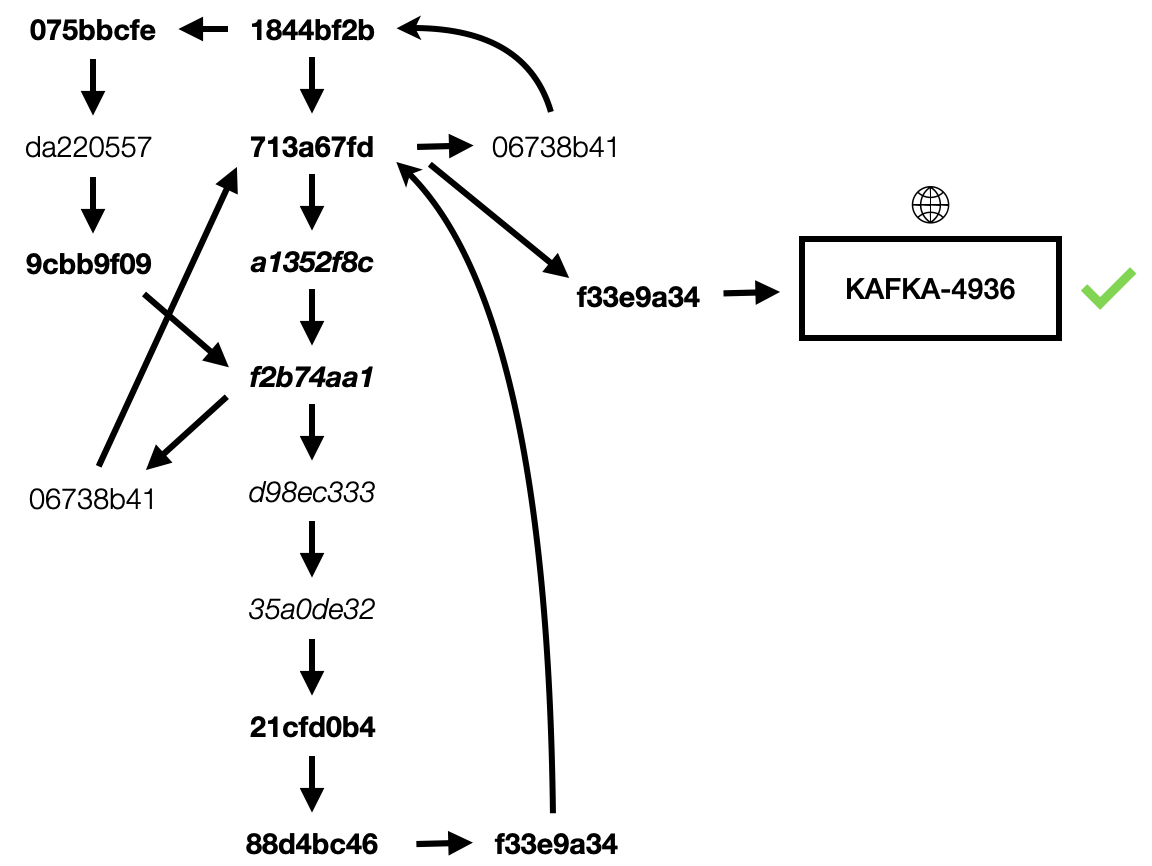
\includegraphics[width=5.5cm]{./images/graph-sample-A.png}}}%
  \qquad
  \subfloat[\centering Participant H's commit history exploration in answering question B(a) \emph{without} Intelligent History. \label{subfig:Exploration-Graph-B}]{{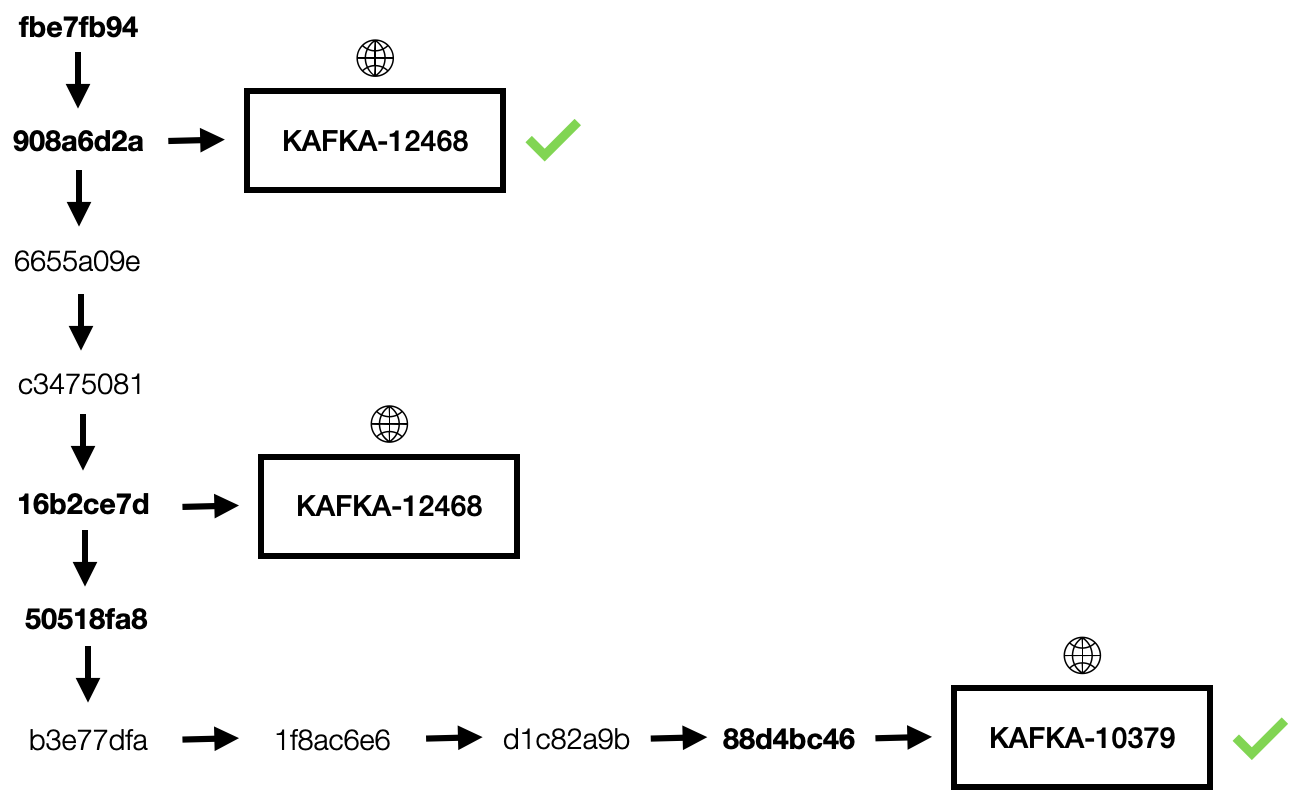
\includegraphics[width=5.5cm]{./images/graph-sample-B.png}}}%
  \caption{
    Commit history exploration graphs.
  }%
  \label{fig:Exploration-Graphs}%
\end{figure}

\begin{figure}
  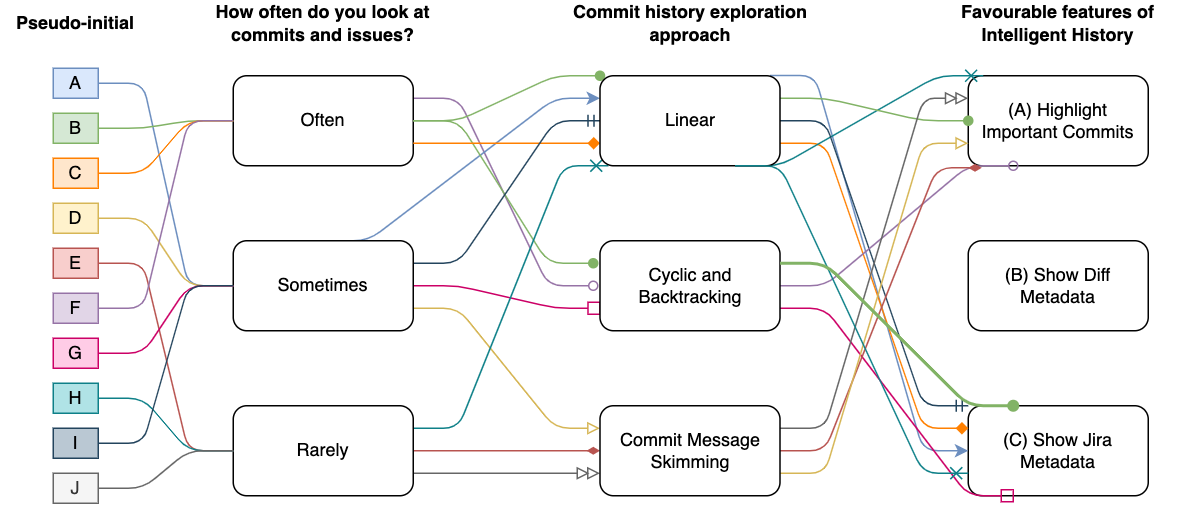
\includegraphics[width=13cm]{./images/flow-chart.png}
  \caption{
    The relationship between how often a participant looks at commits and issues, the approach they exhibited to exploring commit history, and the features of Intelligent History they showed the most enthusiasm for.
  }
  \label{fig:Results-Qualitative}
\end{figure}

\begin{landscape}
  \begin{figure}
    \caption{
      A tabular form of \autoref{fig:Results-Qualitative}.
    }
    \centering
    \begin{tabular}{@{}cccl@{}}
      \toprule
      \textbf{Pseudo-initial} & \textbf{\begin{tabular}[c]{@{}c@{}}How often do you look \\ at commits and issues?\end{tabular}} & \textbf{\begin{tabular}[c]{@{}c@{}}Commit history \\ exploration approach\end{tabular}} & \multicolumn{1}{c}{\textbf{\begin{tabular}[c]{@{}c@{}}Favourable features \\ of Intelligent History\end{tabular}}} \\ \midrule
      A                       & Sometimes                                                                                        & Cyclic and Backtracking                                                                 & (C) Show Jira Metadata                                                                                             \\ \midrule
      B                       & Often                                                                                            & \begin{tabular}[c]{@{}c@{}}Linear\\ Cyclic and Backtracking\end{tabular}                & \begin{tabular}[c]{@{}l@{}}(A) Highlight Important Commits\\ (C) Show Jira Metadata\end{tabular}                   \\ \midrule
      C                       & Often                                                                                            & Linear                                                                                  & (C) Show Jira Metadata                                                                                             \\ \midrule
      D                       & Sometimes                                                                                        & Commit Message Skimming                                                                 & (A) Highlight Important Commits                                                                                    \\ \midrule
      E                       & Rarely                                                                                           & Commit Message Skimming                                                                 & (A) Highlight Important Commits                                                                                    \\ \midrule
      F                       & Often                                                                                            & Cyclic and Backtracking                                                                 & (A) Highlight Important Commits                                                                                    \\ \midrule
      G                       & Sometimes                                                                                        & Cyclic and Backtracking                                                                 & (C) Show Jira Metadata                                                                                             \\ \midrule
      H                       & Rarely                                                                                           & Linear                                                                                  & \begin{tabular}[c]{@{}l@{}}(A) Highlight Important Commits\\ (C) Show Jira Metadata\end{tabular}                   \\ \midrule
      I                       & Sometimes                                                                                        & Linear                                                                                  & (C) Show Jira Metadata                                                                                             \\ \midrule
      J                       & Rarely                                                                                           & Commit Message Skimming                                                                 & (B) Highlight Important Commits                                                                                    \\ \bottomrule
    \end{tabular}
    \label{tab:Results-Quantitative}
  \end{figure}
\end{landscape}

\subsection{RQ1}

\subsection{RQ2}

\subsection{RQ3}

%%%%%%%%%%%%%%%%%%%%%%%%%%%%%%%%%%%%%%%%%%%%%%%%%%%%%%%%%%%%%%%%%%%%%%
\section{Threats to Validity}
\label{sec:Threads-to-Validity}

There are a number of aspects of this user study that impact the construct validity of our results.
Firstly, since the participants were observed throughout the study by the interviewer, the participants' behaviour, opinions, and feedback about the Intelligent History plugin are subject to the Hawthorne effect.

The limited participant size of 10 people affects external validity.

\FIXME{Hawthorne effect, sample size, tool usage for second set of questions -- we did this to mitigate bias or impression of conducting the study a certain way, lack of external validity due to the controlled environment with prescribed questions.}

%%%%%%%%%%%%%%%%%%%%%%%%%%%%%%%%%%%%%%%%%%%%%%%%%%%%%%%%%%%%%%%%%%%%%%
\endinput

Any text after an \endinput is ignored.
You could put scraps here or things in progress.